% Charlotte Geiger - Manuel Lippert - Leonard Schatt
% Physikalisches Praktikum

% Teilauswertung 3
\newpage
\section{Emitterschaltung: Arbeitspunktstabilisierung und Signalverstärkung}
\subsection{Wechselspannungsverstärkung}
\begin{center}
    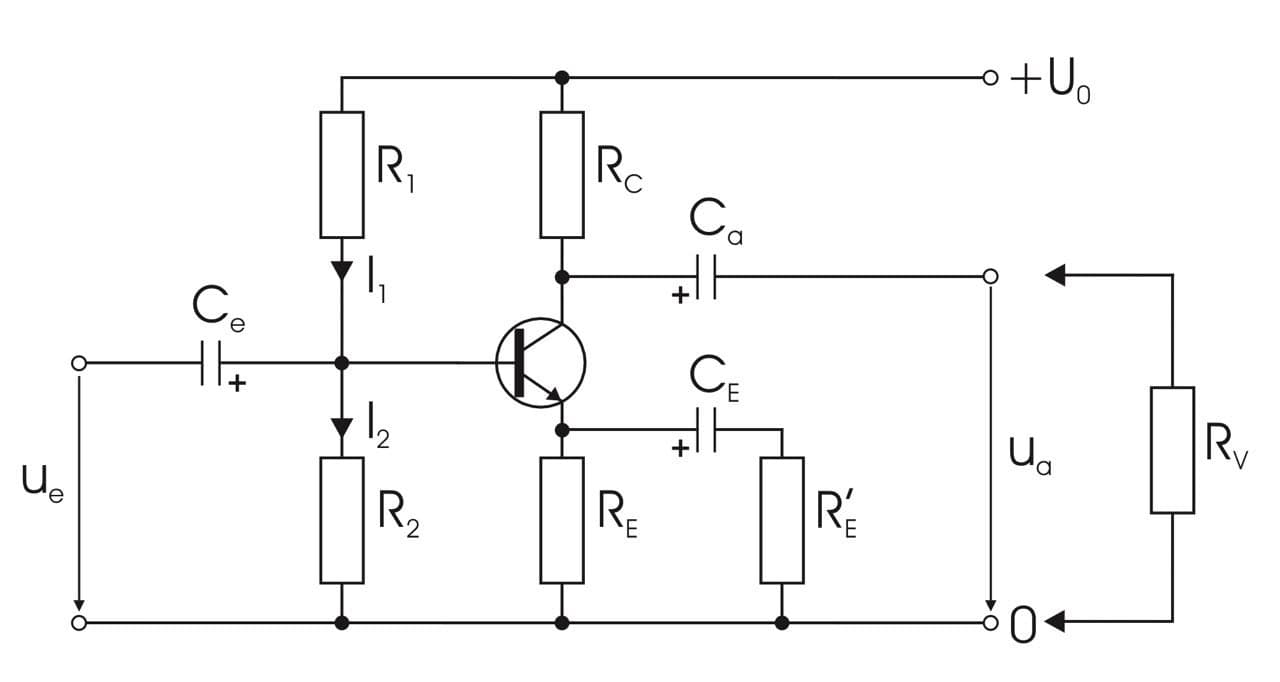
\includegraphics[scale=0.15]{6_3-Emmitterschaltung.jpg}
\end{center}
Betrachtet man die verwendete Schaltung des Versuchs lässt sich folgender Zusammenhang herleiten:
\begin{gather}
    u_e = i_B(R_*+r_{BE})\xrightarrow{R_*\rightarrow~0} i_B r_{BE} \tab R_*=\frac{1}{\frac{1}{R_E}+\frac{1}{R_E' +\frac{1}{i\omega C_e}}} \xrightarrow{R_E,R_E'~\rightarrow~0} 0\\
    u_a = -i_CR_C\tab\text{(Gleichstromanteil = 0)}\\
    \Rightarrow v_3 =\frac{u_a}{u_e}\xrightarrow{R_E,R_E'~\rightarrow~0}-\frac{i_C R_C}{i_B r_{BE}}=-\beta\frac{R_C}{r_{BE}} \tab\text{Gleichung (3)}
\end{gather}
Der Fehler von $v_3$ und folgende Fehler werden mit dem Fehlerfortpflanzungsgesetz ermittelt, wobei der Fehler $s_{R_C}= 28.92~\Omega$ für $R_C=2692~\Omega$ (mit DMM: $0.01 + 2~\text{Digit}$) und $s_{r_{BE}}=0.5~\text{k}\Omega$ für $r_{BE}=4~\text{k}\Omega$. Dabei wurde der Fehler $s_{r_{BE}}$ mit Hilfe anderer Datenblätter abgeschätzt. $\beta = 250$ (Aus Datenblatt) wird als fehlerfrei angenommen.
\begin{gather}
    s_{v_3} = \beta\sqrt{\left(\frac{s_{R_C}}{r_{BE}}\right)^2+\left(\frac{R_C}{r_{BE}^2}s_{r_{BE}}\right)^2}
    %s_{v_3} = \beta\frac{s_{R_C}}{r_{BE}}\\
\end{gather}
\begin{gather*}
    \textcolor{red}{\Rightarrow v_3 = -168.25 \pm 21.1}
\end{gather*}
Die Gleichung (6) aus dem Skript wurde schon in 2.6 hergeleitet und wird hier schon vorrausgesetzt, wobei $R_E=557~\Omega$ mit dem Fehler $s_{R_E}=7.57~\Omega$ gilt.
\begin{gather}
    v_6 =-\frac{R_C}{\frac{r_{BE}}{\beta}+R_E} \\
    s_{v_6} = \sqrt{\left(\frac{s_{R_C}}{\frac{r_{BE}}{\beta}+R_E}\right)^2+ \left(\frac{R_C}{(\frac{r_{BE}}{\beta}+R_E)^2}s_{R_E}\right)^2 + \left(\frac{R_C}{\beta(\frac{r_{BE}}{\beta}+R_E)^2}s_{r_{BE}}\right)^2}
\end{gather}
\begin{gather*}
    \textcolor{red}{\Rightarrow v_6 = -4.70 \pm 0.08}
\end{gather*}
Der Ein- und Ausgangswiderstand lässt sich analog wie in der Dimensionierung berechnet mit $R_1=119.5~\text{k}\Omega$ mit $s_{R_1}=1.4~\text{k}\Omega$ und $R_2=21.86~\text{k}\Omega$ mit $s_{R_2}=0.24~\text{k}\Omega$:
\begin{gather}
    r_e = \frac{1}{\frac{1}{R_1}+\frac{1}{R_2}+\frac{1}{r_{BE}}} \\
    s_{r_e} = r_e^2\sqrt{\left(\frac{s_{R_1}}{R_1^2}\right)^2 + \left(\frac{s_{R_2}}{R_2^2}\right)^2 + \left(\frac{s_{r_{BE}}}{r_{BE}^2}\right)^2}\\
    r_a = R_C \\
    s_{r_a} = s_{R_C}
\end{gather}
\begin{gather*}
    \textcolor{red}{\Rightarrow r_e = (3.29 \pm 0.34)~\text{k}\Omega}\\
    \textcolor{red}{\Rightarrow r_a = (2.70 \pm 0.03)~\text{k}\Omega}
\end{gather*}
Bei der Betrachtung des Temperaturdrifts für $\Delta T = 10~\text{K}$ folgt aus dem Zusammenhang:
\begin{gather}
    \frac{U_0-U_C}{R_C}=I_C\approx I_E=\frac{U_e-U_{BE}}{R_E}\\
    \Rightarrow U_C \approx \frac{R_C}{R_E} U_{BE} +(\frac{U_0}{R_C}-\frac{U_e}{R_E})\\
    \xrightarrow{\frac{\partial}{\partial T}}\frac{\partial U_C}{\partial T}=\frac{R_C}{R_E}\frac{\partial U_{BE}}{\partial T}
\end{gather}
Aus dem Skript wird Gleichung (5) entnommen. Dabei gilt $\frac{\partial U_{BE}}{\partial T}=-2~\frac{\text{mV}}{\text{K}}$ bei konstanten Basisstrom $I_B$.
\begin{align}
    \Rightarrow \Delta U_C = \frac{R_C}{R_E} (-2~\frac{\text{mV}}{\text{K}}) \Delta T 
\end{align}
\begin{align*}
    \textcolor{red}{\Rightarrow \Delta U_C = 96.7~\text{mV}}
\end{align*}

\subsection{Messgrößen am Arbeitspunkt}
Der Fehler für jede gemessene Spannung am Arbeitspunkt werden mit dem Fehler des DMM $s_{\text{DMM}} = 0.08*U + 1~\text{Digit}$ abgeschätzt. Daraus folgen folgende Werte
\begin{center}
    \captionof{table}{Messung am Arbeitspunkt}
    \begin{tabular}{cc|cc|cc}
        $U_C/\text{V}$ & $s_{U_C}/\text{V}$ & $U_B/\text{V}$ & $s_{U_B}/\text{V}$ & $U_E/\text{V}$ & $s_{U_E}/\text{V}$ \\
        \hline
        6.400 & 0.513 & 1.798 & 0.145 & 1.159 & 0.094 \\ 
    \end{tabular}
\end{center}
Mit diesen Werten können wir nun $U_{CE}~U_{BE}~I_C~I_E$ mit den Fehlern (berechnet mit Fehlerfortpflanzungsgesetz):
\begin{gather}
    U_{CE} = U_C - U_E \tab s_{U_{CE}} = \sqrt{s_{U_C}^2+s_{U_E}^2}\\
    U_{BE} = U_B - U_E \tab s_{U_{BE}} = \sqrt{s_{U_B}^2+s_{U_E}^2}\\
    I_C = \frac{U_C}{R_C} \tab s_{I_C} = \sqrt{\left(\frac{1}{R_C}s_{U_C}\right)^2+\left(\frac{U_C}{R_C^2}s_{R_C}\right)^2}\\
    I_E = \frac{U_E}{R_E} \tab s_{I_E} = \sqrt{\left(\frac{1}{R_E}s_{U_E}\right)^2+\left(\frac{U_E}{R_E^2}s_{R_E}\right)^2}
\end{gather}
\begin{center}
    %\captionof{table}{Ergebnis}
    {\color{red}\begin{tabular}{cc|cc|cc|cc}
        $U_{CE}/\text{V}$ & $s_{U_{CE}}/\text{V}$ & $U_{BE}/\text{V}$ & $s_{U_{CE}}/\text{V}$ & $I_C/\text{mA}$ & $s_{I_C}/\text{mA}$ & $I_E/\text{mA}$ & $s_{I_E}/\text{mA}$ \\
        \hline
        5.241 & 0.522 & 0.639 & 0.173 & 2.377 & 0.192 & 2.081 & 0.171 \\ 
    \end{tabular}}
\end{center}
Die berechneten Werten entsprechen den Erwartungen. Am besten kann man dies erkennen an $U_{BE}$ mit dem Wert von $639$ mV, welche davor in der Dimensionierung aus dem Datenblatt mit $650$ mV vorrausgesetzt wurde. Dies ist nicht ganz überraschend, da schon bei der Messung am Versuchstag die Werte aus der Dimensionierung erzielt wurden.

\subsection{Übersteuerung}
Zuerst muss erwähnt werden, dass am Versuchstag vergessen wurde zu dokumentieren in welcher Einstellung das Oszilloskops eingestellt war, weswegen keine genaue Angaben gegen werden können. Im Folgenden wird in nur in Div anstelle von V gesprochen (für V mit entsprechenden Wert multiplizieren).\\ \\
Für die maximale Kollektorspannung $U_C^{\text{max}}$ sperrt der Transistor, wodurch kein Stromfluss mehr möglich ist. Daraus folgt \textcolor{red}{$U_C^{\text{max}} = U_0 = 12~\text{V}$} \\
Bie minimaler C-Spannung lässt der Transistor den maximalen Stromfluss zu. Betrachten wir die Abbildung 4.3 in Kapitel 4.2 so erkennt man, dass bei $U_{CE}\approx 0.7~\text{V}$ der Anstieg des Stromfluss $I_C$ sein Maximum erreicht hat und damit der Strom ungefähr sein MAximalwert erreicht. Woraus folgt, dass sich die restliche Spannung auf den Spannungsteiler verteilt.
\begin{gather}
    \frac{U_0-U_{CE}}{U_C^\text{min}} = \frac{R_E+R_C}{R_E}~\Leftrightarrow~U_C^\text{min}= \frac{R_E}{R_E+R_C}(U_0-U_{CE})\\
    s_{U_C^\text{min}} = \frac{U_C^\text{min}}{R_E+R_C}\sqrt{(s_{R_C})^2+\left(\frac{R_C}{R_E}s_{R_E}\right)^2}
\end{gather}
\begin{align*}
    \textcolor{red}{\Rightarrow U_C^\text{min}=(1.94 \pm 0.03)~\text{V}}
\end{align*}
Bei Betrachtung der Bilder des Oszilloskops wird deutlich, dass die maximale Peak-Peak-Amplitude $U_{pp}^\text{max}$ bei einem ausgebildeten Plateu erreicht ist. Dabei lesen wir $U_{pp}^\text{max}$ von der Nullline des Oszilloskops bis zum Plateu ab.
\begin{gather*}
    U_p^\text{max}=2.3 \pm 0.25~\text{Div} \tab U_p^\text{min}=0.0\pm0.25~\text{Div}\\
    U_{pp}^\text{max} = U_p^\text{max}-U_p^\text{min} \tab s_{U_{pp}^\text{max}}=\sqrt{2}*0.25\\
    \textcolor{red}{\Rightarrow U_{pp}^\text{max}=(2.3 \pm 0.4)~\text{Div}}
\end{gather*}
Anhand der Bilder lässt sich auch erkennen, dass keine symmetrische Übersteuerung bei der positven oder negativen Halbwelle stattfindet, wobei es deutlch ersichtlich ist, dass die positive Halbwelle eine größer Amplitude und ein breiters Plateu besitzt. Bei einer leichten Erhöhung der Eingangsamplitude erkennt man außerdem, dass sich das Plateu zuerst bei der negativen Halbwelle entsteht. Bei kontinuierlicher Erhöhung übersteuert der Versträker und es bildet sich darauf das Plateu in der positiven Halbwelle.
\subsection{Wechslespannungsverstärkung im Vergleich}

Wir tragen die Verstärkung in einem Diagramm auf. Dabei fällt uns erstmal auf, dass wir nichts Auffälliges sehen. Nach eingehendem Studium des Skriptes fällt uns auf, dass 
die Aufgabe vermutlich anders gemeint war. Scheinbar sollte man einen größeren Messbereich messen. Da aufgrund von Infektionsschutzmaßnahmen Nachmessungen bis jetzt immer 
abgelehnt wurden, werten wir die vorhandenen Daten bestmöglich aus.\\
Uns ist jedoch bewusst, dass diese Auswertung höchstenfalls ein unvollständiges Bild geben kann. Die Fehler $s_{u_a}$
nehmen wir wie im Protokoll vermerkt 3\% des gemessen Wertes für das Oszilloskop an und der Ablesefehler beträgt 0.1 Unterteilungen. Für $s_{u_e}$ nehmen wir den Fehler des Frequenzgenerator an.



\begin{table}[h]
    \centering
    \begin{tabular}[h]{c|c|c|c|c|c}


        $u_e/$mV & $u_A/$V & $v$ & $s_{u_e}/$mV&  $s_{u_a}/$V & $s_v$ \\
       \hline
       %Nicht in der Literatur  & 3135 & sdfgsdf \\
        2.5 & 0.4 & 160 & 0.1 & 0.005 & 8 \\
        4.5 & 0.7 & 156 & 0.2 & 0.01 & 8\\
        6.0 & 1.1 & 183 & 0.3 & 0.01 & 9\\
        7.5 & 1.2 & 160 & 0.4 & 0.01 & 8\\
        10.0 & 1.7 & 170 & 0.5 & 0.02 & 9\\
        11.0 & 2.1 & 191 & 0.6 & 0.02 & 10\\
        13.0 & 2.4 & 185 & 0.7 & 0.03 & 9\\
        15.0 & 2.75 & 183 & 0.8 & 0.03 & 9\\
        17.0 & 3.1 & 182 & 0.9 & 0.03 & 9\\
        19.5 & 3.5 179 & 1 & 0.04 & 9\\

       %Nicht in der Literatur  & 8100 & asdf \\
       %Nicht in der Literatur  & 8730 & asdf \\
    \end{tabular}
\end{table}
\begin{figure}[h]
    \centering
    \includegraphics[width = \linewidth]{Bilder/6_4Wechselstromverstärkung1.png}
    \caption{Lineare Regression durch alle Datenpunkte}
\end{figure}
Wenn man durch alle Datenpunkte eine lineare Regression bildet, erkennt man, dass dies keine gute Theorie zu dem Messwerten ist.
Auffällig ist jedoch, dass die Datenpunkt bei $u_e$ größer 10mV einen sehr schönen lineraren Zusammenhang haben. 
Es wäre unserer Meinung nach möglich, dass zumindest für niedrige Werte von $u_e$ ein linearer Zusammenhang besteht. 
Das Abweichen der Messpunkte unter 10 mV könnte an bisher nicht betrachteten Fehlerursachen liegen, welche nur bei niedrigen Eingangsapnnungnen auftreten.
\begin{figure}[h]
    \centering
    \includegraphics[width = \linewidth]{Bilder/6_4Wechselstromverstärkung2.png}
    \caption{Lineare Regression durch Datenpunkte im Bereich 10mV bis 20mV}
\end{figure}

\subsection{Ausgangswiderstand der Emitterschaltung}

Um den Ausgangswiderstand $r_a$ zu ermitteln schließen wir die Widerstandsdekade als Verbraucher an. Da wir $u_a$ kennen (Fall $R_V = \infty$ ) können wir 
$r_a$ auf sehr leicht Art und Weise berechnen. Da wir aus dem Ohm’schen Gesetz wissen, dass bei $R_V = r_a$ die halbe Ausgangsspannung über die Widerstandsdekade 
abfällt folgt, müssen wir nur die Widerstandsdekade so einstellen, dass $u_{R_V} = \frac{u_a}{2}$. Der Fehler setzt sich dabei aus dem Fehler von $R_C$ und dem Fehler der Widerstandsdekade
und dem Ablesefehler zusammen. Der Ablesefehler dominiert hier alle anderen, da es sehr schwer abzulesen war, wann die Spannung genau gleichgroß war. Wir schätzen ihn auf circa 10\%. 
\begin{table}[h!]
    \centering
    \begin{tabular}[h]{c|c||c}
        $r_{a_{gemessen}}/\Omega $ & $s_{r_{a{gemessen}}}/\Omega $ & $r_{a_{gemessen}}/$k$\Omega$\\
       \hline
      
        2500 & 252.3 & \textcolor{red}{2.5$\pm $ 0.3}\\
    \end{tabular}
    \caption{Ausgangswiderstand der Emitterschaltung}
\end{table}
Der gemessene Wert liegt deutlich unter dem errechneten Wert. Dies liegt aber vermutlich 
nur an dem großen Fehler, welcher durch das ungenaue Ablesen entsteht. Der errechnete Wert 
liegt noch in dem Fehlerintervall des gemessenen Wertes.
\subsection{Eingangswiderstand der Emitterschaltung} \label{Eingspa}

Der Eingangswiderstand und sein Fehler lassen sich analog zu den Fragen zur Vorbereitung wieder berechnen durch:
\begin{equation*}
    r_e = [R_{1}^{-1}+R_{2}^{-1}+\frac{1}{r_{BE}+\beta R_E}]^{-1}
\end{equation*}
\begin{equation*}
    s_{r_e} = | r_e |^2 \sqrt{(\frac{s_{R_1}}{R_1^2})^2+(\frac{s_{R_2}}{R_2^2})^2+(\frac{s_{r_{BE}}}{(r_{BE}+\beta R_E)^2} )^2} 
\end{equation*}
Der letzte Term in der Fehlerrechnung geht jedoch für $R_E$ gegen unendlich gegen Null.
Das ergibt wie in Kapitel %@ManeLippert TODO 
berechnet:

\begin{equation*}
    \textcolor{red}{r_e \approx	 (16.5 \pm 0.2)k\Omega}
\end{equation*}
Die Messung wird ähnlich wie in der vorherigen Aufgebe gemacht. Diesmal wird der Widerstand jedoch davor in Reihe geschaltet. Der Fehler wir wieder durch unseren geschätzten 
Ablesefehler dominiert. Dieser liegt hier bei circa 20\%. Die anderen Fehler sind im Vergleich dazu vernachlässigbar.
\begin{table}[h]
    \centering
    \begin{tabular}{c|c||c}
        $r_{e_{gemessen}}$ in k$\Omega$ & $s_{r_{e_{gemessen}}}$ in k$\Omega$ & Ergebnis\\
        \hline
        20 & 4 & \textcolor{red}{(20$\pm $ 4)k$\Omega$}
    \end{tabular}
    \caption{Gemessener Eingangswiederstand}
\end{table}

Der gemessene und der theoretische Wert passen gut zusammen. Es fällt auf, dass der gemessene Wert deutlich 
über dem errechneten liegt. Dies ist jedoch dadurch zu erklären, dass der Fehler der Messung sehr groß ist. 
Der errechnete Wert liegt im Messfehler.

\subsection{Gegenkopplung durch das Verbauen unterschiedlicher $R'_E$}

Schließlich betrachten wir einen algemeineren Fall als das, was wir bis jetzt betrachtet haben. 
Bis jetzt ist $R'_E = \infty$. In diesem Fall verändern wir $R'_E$. Im Grenzfall mit $R'_E$ erwarten wir 
jedoch wieder das selbe wie in Kapitel \glqq \ref{Eingspa}  \titleref{Eingspa}".\\
Im folgenden berechnen wir die erwarteten Werte:\\
\begin{equation*}
    \centering
    r'_e = [\frac{1}{R_1}+\frac{1}{R_2}+\frac{1}{r_{BE}+\beta(\frac{1}{R_E}+\frac{1}{R'_{E}})^{-1}}]^{-1}
\end{equation*}
\begin{equation*}
    \centering
    s_{r'_e} = |r_e|^2 \sqrt{(\frac{s_{R_1}}{R_1^2})^2+(\frac{s_{R_2}}{R_2^2})^2+[r_{BE}+\frac{\beta(R_E+R'_E)}{R_E \cdot R'_E}]^{-4} \cdot [s_{r_{BR}}^2+\frac{\beta^2 s_{R_E}^2}{(R_{E})^4}+(\frac{\beta \cdot s_{R'_E}}{(R'_{E})^2})^2]}
\end{equation*}
Für $R'_E \to \infty$ sind wir im vorherigen Kapitel. Auch die Messwerte sind dabei identisch.\\
Aus dem Formelblatt \footnote{\url{https://docs-emea.rs-online.com/webdocs/0109/0900766b80109ff9.pdf}} entnehmen wir die fü die Rechnung nötigen Daten.
Als Fehler der Messung nehmen wir wieder nur den geschätzten Fehler, da dieser viel größer ist, als die anderen.
\begin{table}[h]
    \centering
    \begin{tabular}{r|c|c|c|c||c||c}
         $n$& $r'_{e,t,n}$ in $\Omega $ & $s_{r'_{e,t,n}}$ in $\Omega $ & $r'_{e,m,n}$ in $\Omega$ & $s_{r'_{e,m,n}}$ in $\Omega $& Ergebnis $r'_t$ & Ergebnis $r'_m$\\
        \hline
        68$\Omega$ & 9920.2762 & 821.359 & 10000 & 2000& \textcolor{red}{(9.9$\pm$0.8)k$\Omega$}& \textcolor{red}{(10$\pm $ 2)k$\Omega$}  \\
        150$\Omega$ &12260.0619 & 1254.500  &22000 & 4400& \textcolor{red}{12$\pm$1)k$\Omega$}& \textcolor{red}{(22$\pm $ 4)k$\Omega$}  \\
        $\infty\Omega$& Siehe & Kapitel& \ref{Eingspa} &  & \textcolor{red}{(16.5 $\pm$ 0.2)k$\Omega$}& \textcolor{red}{(20$\pm $ 4)k$\Omega$}  \\
    \end{tabular}
    \caption{}
\end{table}
Der Messwert bei dem 150$\Omega$ ist eindeutig ein Messfehler. Anders können wir uns einen so hohen Wert nicht erklären. Die anderen beiden Werte passen sehr gut 
zu den theoretisch ermittelten Werten. Bei den theoretischen Werten fallen die großen Fehler auf. Dies lässt sich jedoch durch die Dominanz dieses Thermes im Fehler erklären:
\begin{equation*}
    [r_{BE}+\frac{\beta(R_E+R'_E)}{R_E \cdot R'_E}]^{-4}
\end{equation*}

\subsubsection{Verstärkung mit Gegenkopplungswiderständen}
Die Verstärkung wird aus dem Messwerten wie in den vorherigen Kapiteln berechnet.
Die Verstärkung\footnote{Gleichung (6) im Skript El1} ergibt sich folgendermaßen: 
\begin{equation*}
    v_t = -R_C[\frac{1}{R_E}+\frac{1}{R'_E}] 
\end{equation*}
\begin{equation*}
    s_v = |v_t| \sqrt{(\frac{s_{R_C}}{R_C})^2+(\frac{s_{R_E}}{R_E})^2+(\frac{s_{R'_E}}{R'_E})^2}
\end{equation*}
Mit diesem Formel folgen folgende Werte:\\
\begin{table}[h]
    \centering
    \begin{tabular}{c|c|c}
        Verstärkung & Fehler & Ergenis\\
        \hline
        $v_{m,68}$ = 36 & $s_{v_{m,68}}$ = 1.846& \textcolor{red}{36$\pm$2}\\
        $v_{m,150}$ = 7 & $s_{v_{m,150}}$ = 0.37& \textcolor{red}{7.0$\pm$0.3}\\
        $v_{m,\infty}$ = 5.0 & $s_{v_{m,68}}$ = 0.2695& \textcolor{red}{5.0$\pm$0.3}\\
        \hline
        $v_{t,68}$ = 49.1176 & $s_{v_{t,68}}$ = 2.552227& \textcolor{red}{49$\pm$2}\\
        $v_{t,150}$ = 25.000 & $s_{v_{t,68}}$ = 1.29903& \textcolor{red}{25$\pm$1}\\
        $v_{t,\infty}$ = 5.000 & $s_{v_{t,infty}}$ = 0.25988& \textcolor{red}{5.0$\pm$0.2}\\
    \end{tabular}
\end{table}
Der Wert für den 150$\Omega$ Widerstand ist wie erwartet nicht übereinstimmend. Die anderen Werte passen in der 
Gößenordnung, wobei der untere Wert sehr gut mit dem theoretischen Wert übereinstimmt. Bei großen Werten 
scheint die Theorie nicht mehr ganz mit der Beobachtung übereinzustimmen.